
\documentclass[handout,t]{beamer}
\usepackage[utf8]{inputenc}

\usepackage[alf]{abntex2cite}
\usefonttheme[onlymath]{serif}

\usepackage{graphicx}
\usepackage{caption}
\usepackage{float}
\usepackage{geometry}
\usepackage{amsmath,amssymb,lmodern, lipsum}
\usepackage{url}
\usepackage{pgfpages}
\usepackage{enumerate}
\usepackage{color}
\usepackage{ifthen}
\usepackage{capt-of}
\usepackage{listings}
\usetheme{Berlin}
\usecolortheme{ufrn}
\usepackage{soul}
\usepackage{algorithm,algorithmic}
\usepackage{romannum}
%\usepackage{enumitem}
\usepackage[export]{adjustbox}

%\usepackage[backend=bibtex]{biblatex}
%\addbibresource{bib/references.bib}

\newcommand{\comment}[1]{}

\setbeamertemplate{caption}[numbered]

\title[Deep Neural Networks Basics]{
	Introduction to Deep Learning for Scientists and Engineers}
\date{
	\today}
\author[Abhijat Vatsyayan]{
%	Abhijat Vatsyayan \inst{1}\\
	Abhijat Vatsyayan
}

\comment{
	\institute[ Enterprise Information Strategy and Risk Management,]{
		\inst{1}%
		EIM\\	
		\href{http://iamap.bms.com}{http://iamap.bms.com}
	}
}
\definecolor{mygreen}{rgb}{0,.5,.1}
\lstset{
	basicstyle=\tiny, 
	%size=10,
	language=Java, 
	commentstyle=\color{mygreen},    % comment style
	escapeinside={\%*}{*)},          % if you want to add LaTeX within your code
	extendedchars=true,              % lets you use non-ASCII characters; for 8-bits encodings only, does not work with UTF-8
	frame=single,	                   % adds a frame around the code
	keepspaces=true,                 % keeps spaces in text, useful for keeping indentation of code (possibly needs columns=flexible)
	keywordstyle=\color{blue},       % keyword style
	morekeywords={*,...},            % if you want to add more keywords to the set
	numbers=left,                    % where to put the line-numbers; possible values are (none, left, right)
	numbersep=5pt,                   % how far the line-numbers are from the code
	numberstyle=\tiny\color{gray}, % the style that is used for the line-numbers
	rulecolor=\color{black},         % if not set, the frame-color may be changed on line-breaks within not-black text (e.g. comments (green here))
	showspaces=false,                % show spaces everywhere adding particular underscores; it overrides 'showstringspaces'
	showstringspaces=false,          % underline spaces within strings only
	showtabs=false,                  % show tabs within strings adding particular underscores
	stepnumber=2,                    % the step between two line-numbers. If it's 1, each line will be numbered
	stringstyle=\color{red}
	}
\begin{document}
	
\setlength{\abovedisplayskip}{0pt}
\setlength{\belowdisplayskip}{0pt}
\setlength{\abovedisplayshortskip}{0pt}
\setlength{\belowdisplayshortskip}{0pt}

\frame{\titlepage}
\section[]{}
\begin{frame}{Summary}
	\tableofcontents
\end{frame}

\section{Introduction}

\begin{frame}{Fitting a function to data}
		\begin{block}{Description (supervised learning)}
		Given a set of data $(x_1,y_1),(x_2,y_2), \dots, (x_n,y_n)$, can 
		we find a function $y=f(x)$ that "fits" this data? 		
		\end{block}		
		\begin{block}{Questions}
			\begin{itemize}
				\item What is this function $f(x)$?
				\item What does "fit" mean? 
				\item How do we know this works? 
				\item What kinds of problems can we solve? 
			\end{itemize}
		\end{block}
\end{frame}

\begin{frame}{More about $f(x)$}
	\begin{block}{Class of functions} 
		Starting with a function $f(x;\theta_1,\theta_2,\dots, \theta_n)$
		where $x$ is the input to the function and $\theta s$ are its parameters, 
		we need to find the set of $\theta s$ that best "fits" the give 
		data $(x_1,y_1),(x_2,y_2), \dots, (x_n,y_n)$ 
		
	\end{block}
	\begin{block}{Class of linear functions}
		Consider  $f(x) = ax+b$. If we can say, with some confidence, that 
		our data is linearly related,  we need to find  
		$\theta_1=a$, $\theta_2=b$ that {\it fits} the given data. 
		We can also write it as $f(x;a,b) = ax+b$. 
	\newline 
	Preferred,  
	\begin{align}
	f(x;\theta_1,\theta_2) &=& \theta_1x+\theta_2	
	\end{align}

	\end{block}

\end{frame}
\begin{frame}{Fit}
	\begin{block}{Squared Euclidean distance as one possible measure of fit}
		Let $L_i$ be the squared Euclidean distance between the predicted 
		value, $\hat{y_i}=f(x_i)$ and the actual, $y_i$. Then,  
		\begin{align}
		L_i &=&z_i^2 \\
		z_i &=&y_i-f(x_i)\\
		    &=&y_i-\theta_1 x_i-\theta_2 
		\end{align}
		Minimizing $L_i$ with respect to the parameters $\theta_1$ and $\theta_2$,
		\begin{align}
		\frac{\partial L_i}{\partial \theta_1} &=& 
		\frac{\partial z_i^2}{\partial z_i} \; 
		\frac{\partial z_i}{\partial \theta_1}  \\
		\frac{\partial L_i}{\partial \theta_2} &=& 
		\frac{\partial z_i^2}{\partial z_i} \; 
		\frac{\partial z_i}{\partial \theta_2}  \\
		\end{align}
	\end{block}
\end{frame}


%\section{Notations}
\begin{frame}{Matrix multiplication as a function}
		\begin{block}{$x \in \mathbb{R}^n$,$y \in \mathbb{R}^m$, $w\in \mathbb{R}^{m \times n}$}
			\begin{align*}
				\begin{bmatrix}
					y_1 \\
					y_2 \\
					\vdots \\
					y_m
				\end{bmatrix} & =  
				\begin{bmatrix}
					w_{11} & w_{12}& \dots & w_{1n}  \\
					w_{21} & w_{22}& \dots & w_{2n}  \\
					\vdots &\vdots &  & \vdots  \\
					w_{m1} & w_{m2}& \dots & w_{mn}  \\
				\end{bmatrix}
			\begin{bmatrix}
				x_1 \\
				x_2 \\
				\vdots \\
				x_n
			\end{bmatrix} \\
		\vec{y} &=w\vec{x} \\
			\end{align*}

		\end{block}
\end{frame}
\begin{frame}{Derivatives}
	For $m=2, n=3$
	\begin{align}
		y_1 &= w_{11}x_1 + w_{12}x_2+w_{13}x_3  \\
		y_2 &= w_{21}x_1 + w_{22}x_2+w_{23}x_3  \\ 
		\begin{bmatrix}
			\frac{\partial y_1}{\partial x_1} & 
				\frac{\partial y_1}{\partial x_2}& 
				\frac{\partial y_1}{\partial x_3}  \\
			\frac{\partial y_2}{\partial x_1}  & 
				\frac{\partial y_2}{\partial x_2}  & 
				\frac{\partial y_2}{\partial x_3}  
		\end{bmatrix} &= 
		\begin{bmatrix}
			w_{11} &  w_{12} & 	w_{13} \\
			w_{21} &  w_{22} & 	w_{23} 
		\end{bmatrix} \\
		\frac{d\vec{y}}{d\vec{x}} &=w 
	\end{align}
\end{frame}
\begin{frame}{Element wise operations}
	\begin{align}
	\sigma(x)  &= \frac{1}{1+e^{-x}}  \\
	%%%%%%%%%%%%
	\frac{d}{d x}\sigma(x) & =  \sigma(x) (1-\sigma(x)) \\
	%%%%%%%%%%%
	\sigma(
		\begin{bmatrix}
			z_1 \\
			z_2 \\
			\vdots \\
			z_m
		\end{bmatrix}
	) & = 
	\begin{bmatrix}
		\sigma(z_1) \\
		\sigma(z_2) \\
		\vdots \\
		\sigma(z_m)
	\end{bmatrix}
	\end{align}
\end{frame}

\begin{frame}{Computation graph } 
	\begin{block}{ Partial derivatives of $f(x,y,z)= sin(x^2y)+e^z$}
		\begin{align}
			\frac{\partial f}{\partial x} &= 2xycos(x^2y) \\
			\frac{\partial f}{\partial y} &= x^2cos(x^2y) \\
			\frac{\partial f}{\partial z} &= e^z 
		\end{align}
	\end{block}
\end{frame} 

\begin{frame}{Computation graph}
	\begin{block}{ Compute graph of $f(x,y,z)= sin(x^2y)+e^z$}
		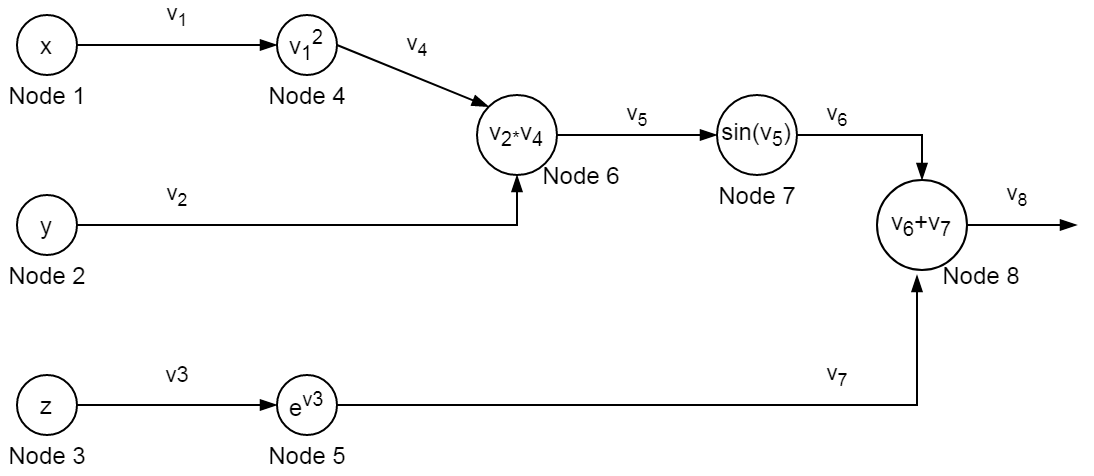
\includegraphics[width=1.\textwidth, center]{figuras/backprop_eg1.png}
	\end{block}
\end{frame}

\begin{frame}{Unit operations (and a little bit of python)\cite{DBLP:journals:corr:BaydinPR15:2018}}
\begin{columns}
	\begin{column}{.5\textwidth}
		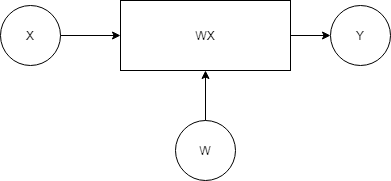
\includegraphics[width=.9\textwidth, center]{figuras/wx_forward_pass.png}
		\lstinputlisting[language=Python, basicstyle=\tiny]{code/MultLayer.py}
	\end{column}
	\begin{column}{.5\textwidth}
		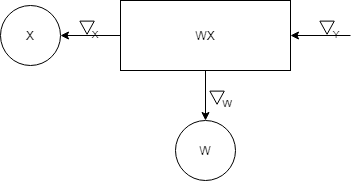
\includegraphics[width=.9\textwidth, center]{figuras/wx_backward_pass.png}
		\lstinputlisting[language=Python, basicstyle=\tiny]{code/AddLayer.py}
	\end{column}
\end{columns}
\comment{
{\tiny
	\lstinputlisting[language=Python]{code/MultLayer.py}
}}
\end{frame}

\begin{frame}{}
	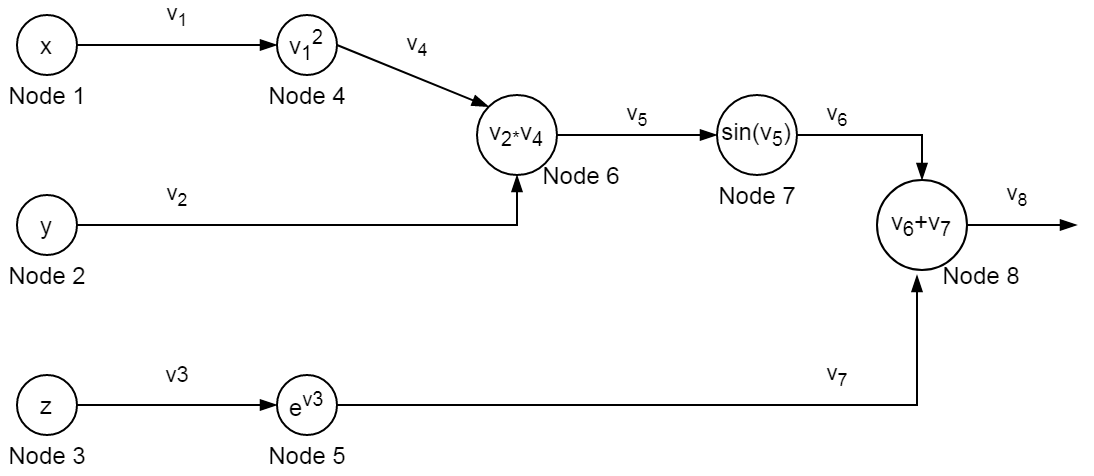
\includegraphics[width=.7\textwidth, center]{figuras/backprop_eg1.png}
	\begin{columns}[T]
		\begin{column}{.5\textwidth}
		
			\begin{align*}
					\frac{\partial v_8}{\partial z}&= 
					\frac{\partial v_8}{\partial v_7} 
					\frac{\partial v_7}{\partial v_3} 
					\frac{\partial v_3}{\partial z}  \\
					&= 1.e^{v_3}.1 \\
					\frac{\partial v_8}{\partial z}&=\frac{\partial f}{\partial z} 
					= e^{v_3}=e^z 
			\end{align*}
		\end{column}
		\begin{column}{.5\textwidth}
			\begin{align*}
			\frac{\partial v_8}{\partial y}&= 
			\frac{\partial v_8}{\partial v_6} 
			\frac{\partial v_6}{\partial v_5} 
			\frac{\partial v_5}{\partial v_2}  
			\frac{\partial v_2}{\partial y}\\
			& = 1.cos(v_5).v^4.1 \\
			\frac{\partial f}{\partial y}&=\frac{\partial v_8}{\partial y}
			= cos(v_5)v^4 \\
			&= cos(v_2v_4)v_4 \\
			&= cos(v^2_1y)v^2_1 \\
			&= cos(x^2y)x^2
			\end{align*}
		\end{column}
	\end{columns}
\end{frame}
\section{Fitting functions}

\begin{frame}{Fitting a function to data}
		\begin{block}{Description (supervised learning)}
		Given a set of data $(x_1,y_1),(x_2,y_2), \dots, (x_n,y_n)$, can 
		we find a function $y=f(x)$ that "fits" this data? 		
		\end{block}		
		\begin{block}{Questions}
			\begin{itemize}
				\item What is this function $f(x)$?
				\item What does "fit" mean? 
				\item How do we know this works? 
				\item What kinds of problems can we solve? 
			\end{itemize}
		\end{block}
\end{frame}

\begin{frame}{More about $f(x)$}
	\begin{block}{Class of functions} 
		Starting with a function $f(x;\theta_1,\theta_2,\dots, \theta_n)$
		where $x$ is the input to the function and $\theta s$ are its parameters, 
		we need to find the set of $\theta s$ that best "fits" the give 
		data $(x_1,y_1),(x_2,y_2), \dots, (x_n,y_n)$ 
		
	\end{block}
	\begin{block}{Class of linear functions}
		Consider  $f(x) = ax+b$. If we can say, with some confidence, that 
		our data is linearly related,  we need to find  
		$\theta_1=a$, $\theta_2=b$ that {\it fits} the given data. 
		We can also write it as $f(x;a,b) = ax+b$. 
	\newline 
	Preferred,  
	\begin{align}
	f(x;\theta_1,\theta_2) &= \theta_1x+\theta_2	
	\end{align}

	\end{block}

\end{frame}
\begin{frame}{Fit}
	\begin{block}{Mean squared Euclidean distance as one possible measure of fit}
		Let $L_i$ be the squared Euclidean distance between the predicted 
		value, $\hat{y_i}=f(x_i)$ and the actual, $y_i$. Then,  
		\begin{align}
		L_i &=z_i^2 \\
		z_i &=y_i-f(x_i)\\
		    &=y_i-\theta_1 x_i-\theta_2 
		\end{align}
		Minimizing $L_i$ with respect to the parameters $\theta_1$ and $\theta_2$,
		\begin{align}
		\frac{\partial L_i}{\partial \theta_1} &= 
		\frac{\partial z_i^2}{\partial z_i} \; 
		\frac{\partial z_i}{\partial \theta_1}  \\
		\frac{\partial L_i}{\partial \theta_2} &= 
		\frac{\partial z_i^2}{\partial z_i} \; 
		\frac{\partial z_i}{\partial \theta_2} 
		\end{align}
	\end{block}
\end{frame}

\begin{frame}%{Mean squared distance and fit}
	For $n$ data points, mean  loss is 
	\begin{align*}
		L = \frac{1}{n} \sum_{i=1}^{i=n}L_i  
		  = \frac{1}{n} \sum_{i=1}^{i=n} (y_i-\theta_1 x_i-\theta_2)^2
	\end{align*}
	In practice
	\begin{itemize}
		\item Choose a small (64 or 128) random subset of training data. 
		\item Compute predicted values, then loss.
		\item Compute gradients of parameters W.R.T. loss and update parameters. 
	\end{itemize}
	An  {\bf epoch} refers to a single iteration over all training data.
	\begin{block}{Two different spaces}
		\begin{itemize}
			\item Space spanned by $x$ and $y$. Optimization tries to find the surface (model) 
			in this space that best fits the data. 
			\item Space spanned by $\theta s$. We minimize the loss function in this space.  
		\end{itemize}
	\end{block}
\end{frame}



\section{Adding non-linearity}
\begin{frame}{Using sigmoid}
	\begin{block}{Definition}
		\begin{align}
			\sigma(x)  &= \frac{1}{1+e^{-x}}  \\
			\frac{d}{d x}\sigma(x) & =  \sigma(x) (1-\sigma(x))
		\end{align}
	\end{block}
	\begin{block}{Assuming a non-linear function}
		Let our function be $y=\sigma(\theta_1 x+\theta_2)$. 
	\end{block}
\end{frame}
\begin{frame}{Making a non-linear function}
	\begin{block}{New function and the squared error}  
	\begin{align}
	z&=\sigma(\hat{y}) \\
	\hat{y} &= \theta_1 x+\theta_2  
	\end{align}
	Error $L_i$ for the ith data point 
	
	\begin{align}
	L_i&=(\sigma(\theta_1 x_i+\theta_2) - y_i)^2   
	\end{align}
	
\end{block}
\end{frame}
\begin{frame}{Finding best $\theta$s}
\begin{block}{Minimizing $L_i$}
	\begin{align}
		L_i &=\Delta_i^2 \\
	\Delta_i &= z_i-y_i \\
	z_i&=\sigma(\hat{y_i}) \\
	\hat{y_i} &= \theta_1 x_i+\theta_2  \\
	%%%%%%%%%%%%%%%%%%%%%%%%%%%%%%%%%%%%%%%%%%%%%%%%%
	\frac{\partial L_i}{\partial \theta_1} &=
	\underbrace{ 
	\frac{\partial \Delta_i^2}{\partial \Delta_i} \; 
	\frac{\partial \Delta_i}{\partial z_i}  \;
	\frac{\partial z_i}{\partial \hat{y_i}} }\;
	\frac{\partial \hat{y_i}}{\partial \theta_1} \\
	%%%%%%%%%%%%%%%%%%%%%%%%%%%%%%%%%%%%%%%%%%%%%%%
	\frac{\partial L_i}{\partial \theta_2} &=
	\underbrace{ 
	\frac{\partial \Delta_i^2}{\partial \Delta_i} \;  
	\frac{\partial \Delta_i}{\partial z_i}  \;
	\frac{\partial z_i}{\partial \hat{y_i}} } \;
	\frac{\partial \hat{y_i}}{\partial \theta_2} 
	\end{align}
\end{block}
\end{frame}
\begin{frame}{Finding best $\theta$s}
\begin{block}{Updates to $\theta_1$ and $\theta_2$}
	\begin{align}
	\frac{\partial L_i}{\partial \theta_1} &=
	\underbrace{ 
		\frac{\partial \Delta_i^2}{\partial \Delta_i}  
		\frac{\partial \Delta_i}{\partial z_i}  
		\frac{\partial z_i}{\partial \hat{y_i}} }
	\frac{\partial \hat{y_i}}{\partial \theta_1} \\
	%%%%%%%%%%%%%%%%%%%%%%%%%%%%%%%%%%%%%%%%%%%%%%%%%%
	\frac{\partial L_i}{\partial \theta_2} &=
	\underbrace{ 
		\frac{\partial \Delta_i^2}{\partial \Delta_i}  
		\frac{\partial \Delta_i}{\partial z_i}  
		\frac{\partial z_i}{\partial \hat{y_i}} }
	\frac{\partial \hat{y_i}}{\partial \theta_2} \\
	%%%%%%%%%%%%%%%%%%%%%%%%%%%%%%%%%%%%%%%%%%%%%%%%%%%
	\theta_{1_{p+1}} &= \theta_{1_p} - \eta \frac{\partial L_i}{\partial \theta_1} \\
	\theta_{2_{p+1}} &= \theta_{2_p} - \eta \frac{\partial L_i}{\partial \theta_2} 
	\end{align}
\end{block}
\end{frame}

\begin{frame}{Finding best $\theta$s}
\begin{block}{Updates to $\theta_1$ and $\theta_2$}
	\begin{align}
	%%%%%%%%%%%%%%%%%%%%%%%%%%%%%%%%%%%%%%%%%%%%%%%%%%%
	\theta_{1_{p+1}} &= \theta_{1_p} - \eta \frac{\partial L_i}{\partial \theta_1} \\
	\theta_{2_{p+1}} &= \theta_{2_p} - \eta \frac{\partial L_i}{\partial \theta_2}  
	\end{align}
\end{block}
\begin{block}{Vectorized format}
	\begin{align}
	\vec{\theta_{p+1}} & =  \vec{\theta_p} - \eta \vec{\nabla_\theta L}
	\end{align}
\end{block}
\end{frame} 
\section{Multi dimensional inputs and outputs}
\begin{frame}{Using vectors}

		\begin{block}{$x \in \mathbb{R}^n$,$y \in \mathbb{R}^m$, $w\in \mathbb{R}^{m \times n}$}
			\begin{align*}
				\begin{bmatrix}
					y_1 \\
					y_2 \\
					\vdots \\
					y_m
				\end{bmatrix} & =  
				\begin{bmatrix}
					w_{11} & w_{12}& \dots & w_{1n}  \\
					w_{21} & w_{22}& \dots & w_{2n}  \\
					\vdots &\vdots &  & \vdots  \\
					w_{m1} & w_{m2}& \dots & w_{mn}  \\
				\end{bmatrix}
			\begin{bmatrix}
				x_1 \\
				x_2 \\
				\vdots \\
				x_n
			\end{bmatrix} + 
			\begin{bmatrix}
			b_1 \\
			b_2 \\
			\vdots \\
			b_n
			\end{bmatrix}
			\end{align*}
		For $m=2, n=3$
		\begin{align}
		y_1 &= w_{11}x_1 + w_{12}x_2+w_{13}x_3 + b_1 \\
		y_2 &= w_{21}x_1 + w_{22}x_2+w_{23}x_3 + b_2 
		\end{align}
		\end{block}
\end{frame}
\begin{frame}{Mandatory network diagram}
	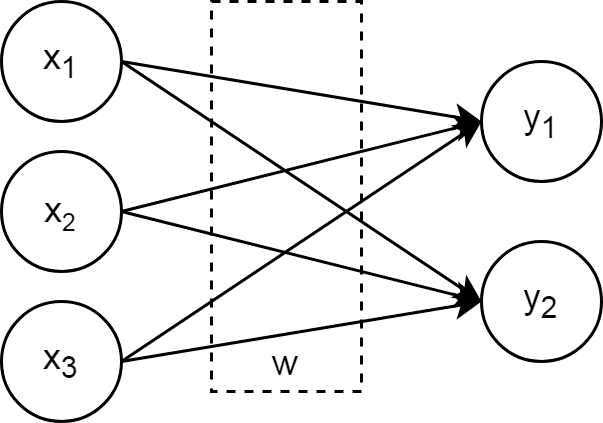
\includegraphics[width=.6\textwidth, center]{figuras/fully_connected_0_layer.png}	
\end{frame}
\begin{frame}{More layers}
	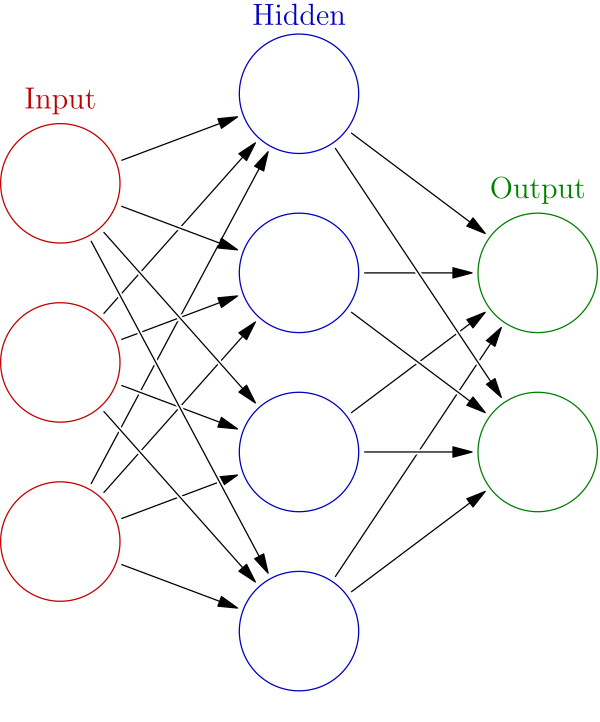
\includegraphics[width=.5\textwidth, center]{figuras/Colored_neural_network_1_hidden.png}
	\tiny{Image from https://en.wikipedia.org/wiki/Artificial\_neural\_network }
\end{frame}
\section{Multi-layer networks with non-linearity}
\begin{frame}{Multiple layers}
	\begin{block}{Layers (composition) of $ax+b$ style functions}
		
\includegraphics[width=.5\textwidth, center]{figuras/two_layer_simple.png}
		\begin{align*}
		y &= \mathbb{W} x + b  \\
		z &= \mathbb{U} y + c =\mathbb{U}(\mathbb{W}x+b)+c \\
		  &= (\mathbb{U}\mathbb{W})x + (\mathbb{U}b+c) = \mathbb{V}x+d 
		\end{align*}
	\end{block}
	\begin{block}{Introducing non-linearity with element-wise sigmoid}
		\begin{align*}
		y &= \sigma(\mathbb{W} x + b) \\ 
		z &= \sigma(\mathbb{U} y + c) 
		\end{align*}
	\end{block}
\end{frame}

\begin{frame}{What can these functions (neural networks) do?}
\begin{quote}
	{\small
		A standard multilayer feed-forward network with a locally bounded 
		piecewise continuous activation function can approximate any continuous 
		function to any degree of accuracy if and only if the network's activation 
		function is not a polynomial.\\
		-Leshno et al.,1993
	}
\end{quote}
\begin{quote}
	{\small 
		In particular, we show that arbitrary decision regions can
		be arbitrarily well approximated by continuous feed forward neural networks with
		only a single internal, hidden layer and any continuous sigmoidal nonlinearity.\\
		-Cybenko, 1989 
	}
\end{quote}
\end{frame}

\begin{frame}{Multi-layer, feed forward, non-polynomial}
		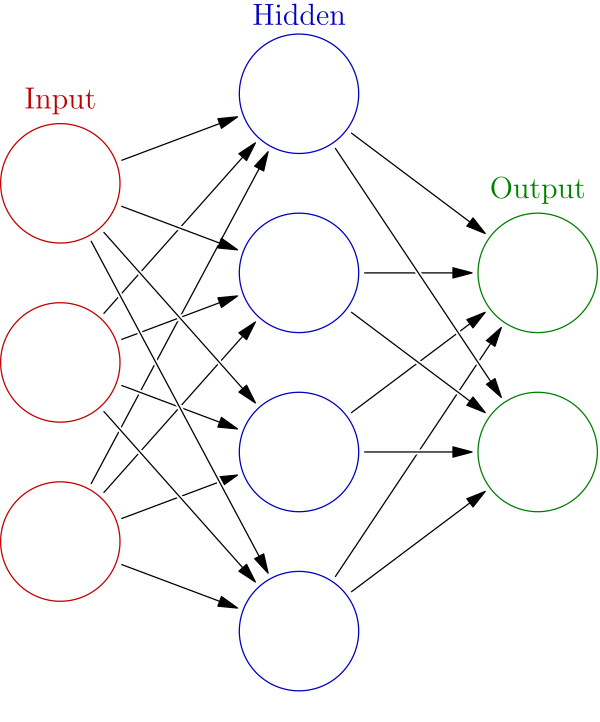
\includegraphics[width=.4\textwidth, center]{figuras/Colored_neural_network_1_hidden.png}
		\tiny{Image from https://en.wikipedia.org/wiki/Artificial\_neural\_network }	
\end{frame}

\begin{frame}{Activation functions}
	\begin{columns}[T]
		\begin{column}{.5\textwidth}
			\tiny{
				\[
				f(x)=\frac{1}{1+e^{-x}}
				\]
			}
			\begin{figure}
				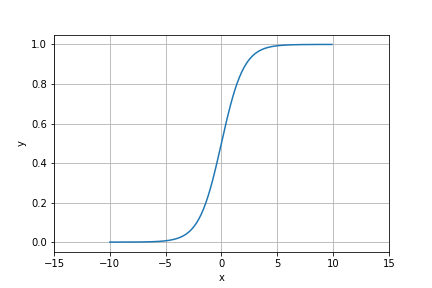
\includegraphics[width=.6\textwidth, center]{figuras/sigmoid.png}	
			\end{figure}
			\tiny{
				\[
				f(x)=\frac{e^x-e^{-x}}{e^x+e^{-x}}
				\]
			}
			\begin{figure}
				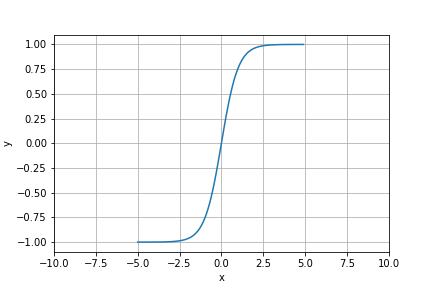
\includegraphics[width=.6\textwidth, center]{figuras/tanh.png}
			\end{figure}
		\end{column}
	%%
		\begin{column}{.5\textwidth}
			\tiny{
				\[
				f(x)=max(x,0)
				\]}
			\begin{figure}
				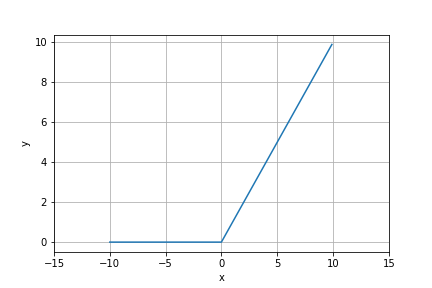
\includegraphics[width=.6\textwidth, center]{figuras/relu.png}	
			\end{figure}
			\tiny{
				\[
				f(x)= 
				\begin{cases}
					x,& \text{if } x\geq 0\\
					0.1x,              & \text{otherwise}
				\end{cases}
				\]
			}
			\begin{figure}
				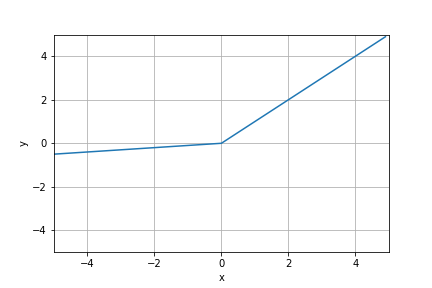
\includegraphics[width=.6\textwidth, center]{figuras/leaky_relu.png}	
			\end{figure}
		\end{column}
	\end{columns}
\end{frame}


\begin{frame}{Why now?}
\begin{itemize}
	\item Activation functions 
	\item Initialization approaches
	\item New optimization algorithms$^*$ 
	\item Architectures for better propagation of gradients 
	\item Availability of massive amounts of data - generation + storage 
	\item Advances in processor speeds and GPUs 
\end{itemize}
\end{frame}

\section{Using what we have seen so far}
\begin{frame}{Steps}
	\begin{itemize}
		\item<1> Settle on a class of function with parameters to be optimized
		 
		\item<-2> Define a secondary function - the loss function. 
		 
		\item<-3> Split data into two sets, a training set and a test set. 
	  
		\item<-4> Optimize the loss function  to find the {\it best} parameters using 
		the training set. 
		
		\item<-5> Use test set to see how well your function with it's parameter work.
	\end{itemize}
\end{frame}
\section{References}
\begin{frame}
\frametitle{References}
\footnotesize{
	\begin{thebibliography}{99}
		\bibitem[Baydin 2018]{p1} Automatic differentiation in machine learning: A survey\\
		\newblock Atilim Gunes Baydin, Barak A. Pearlmutter \& Alexey Andreyevich Radul
		\newblock \emph{arxiv} http://arxiv.org/abs/1502.05767
		
	\end{thebibliography}
}
\end{frame}



\end{document}
